\section{Correlation analysis with data reduction}

\subsection{Choice between PCA and t-SNE}
By looking at the matrix plot, we can see that a lot of variables are correlated. We can exclude from our analysis the 3 colomns: T, RH and AH because there are the less correlated

We decided to use PCA for the correlation analysis because it is a deterministic algorithm and we can reproduce the same results. 
We know that PCA is not the best algorithm in general but in our case, our data are very correlate so this method work really well in our case. 
A very good thing with PCA is that there isn't any hyperparameter to tune the algorithm is so much more easy to use than t-SNE.

\begin{figure}[h]
\centering
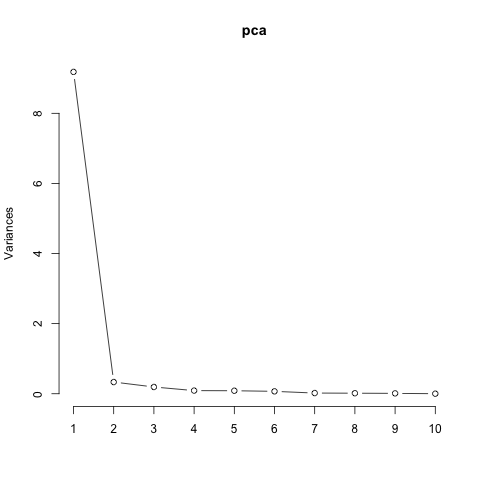
\includegraphics[width=0.5\textwidth]{figs/pca.png}
\caption{Scree plot of the PCA}
\label{fig:scree_plot}
\end{figure}

\subsection{2D plot of the data}


\begin{figure}[H]
\centering
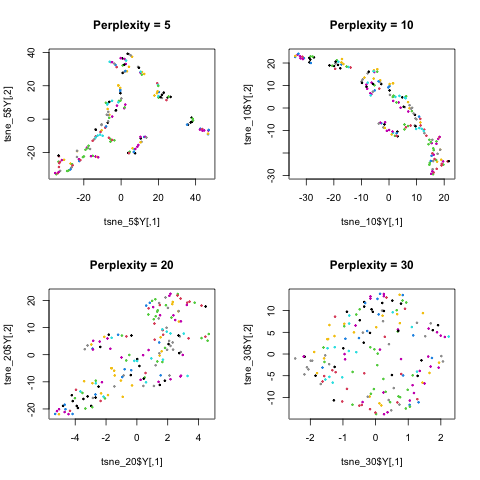
\includegraphics[width=0.5\textwidth]{figs/tsne.png}
\caption{2D plot of the data}
\label{fig:2d_plot}
\end{figure}
